% atifcppprogrammers's Data Communication Lab Report %
\documentclass[fullpage]{article}
\usepackage{tgpagella}
\usepackage{graphicx}
\usepackage{float}
\usepackage[english]{babel}
\usepackage[latin1]{inputenc}

\begin{document}

   \title{Experiment 2 - Introduction to Network Simulator Version-3 (NS-3)}

   \author{Muhammad Atif Farooq L144392 EL-A}

   \date{12th September 2019}

   \maketitle

\section{Introduction}
NS-3 is an open-source discrete-event network simulator for internet systems,
built using C++ and Python. It is used primarily for research and educational
purposes and is publicly available for use under the GNU GPLv2 license.

\section{Objective}
To build and analyze a simple point to point link topolgy in NS-3.

\section{Procedure}
Before discussing the procedure we must remark that the following experiment was
performed on a linux machine using the Ubuntu 18.04 LTS distribution. We now discuss the expermiment 
in the following sections starting out with the installation and build.

\subsection{Installing and Building NS-3}
To Install NS-3 we proceed to the link \verb|https://www.nsnam.org/releases| and download
the latest release as a tarball compressed file. As of this writing \verb|ns-3.30| is the latest
release thus we use it as our reference. Upon a successful download extract the file into
your preferred directory and enter the extracted \verb|ns3-allinone| directory using your terminal.
Finally execute \verb|build.py| script using \verb|./build.py --enable-examples --enable-tests|
and wait until all required packages are installed.

\subsection{Building and Executing Scripts}
Having built NS-3, copy the \verb|first.cc| file present in \verb|examples/tutorials|
and paste it in the the \verb|scratch| directory, following this navigate back to the
\verb|ns-3.30| directory and execute the \verb|./waf --run scratch/first| command
inside the \verb|ns-3.30| directory to build and run the \verb|first.cc| script.To run your own
scripts write them inside the \verb|scratch| directory and follow the remaining procedure as
stated above. You should see the following output on your terminal, after executing
\verb|./waf --run scratch/first|.

\begin{figure}[h!]
  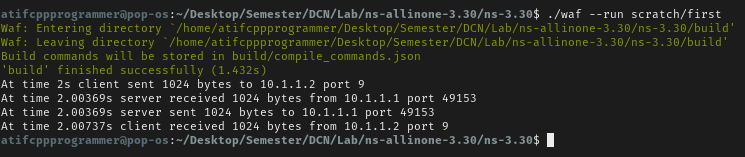
\includegraphics[width=\linewidth]{runFirst.png}
  \caption{first.cc}
  \label{fig:output1}
\end{figure}

\subsection{Task}

As directed by the manual we first commented on the output of the \verb|first.cc| script
presented in Figure-1 which indicates that the client intiates the communication by sending a
packet to the server, the server then receives the said packet, and then sends packet of its
own to the client acknowledging that the original packet was successfully received by it.

The Lab task also required us to modify the above code, to change the packet size, data rate,
transmisson delay, IP addressing of the nodes and the server port. The Code and its accompanying output
are presented below.

\begin{verbatim}

#include "ns3/core-module.h"
#include "ns3/network-module.h"
#include "ns3/internet-module.h"
#include "ns3/point-to-point-module.h"
#include "ns3/applications-module.h"

using namespace ns3;

NS_LOG_COMPONENT_DEFINE ("FirstScriptExample");

int
main (int argc, char *argv[])
{
  CommandLine cmd;
  cmd.Parse (argc, argv);

  Time::SetResolution (Time::NS);
  LogComponentEnable ("UdpEchoClientApplication", LOG_LEVEL_INFO);
  LogComponentEnable ("UdpEchoServerApplication", LOG_LEVEL_INFO);

  NodeContainer nodes;
  nodes.Create (2);

  PointToPointHelper pointToPoint;
  pointToPoint.SetDeviceAttribute ("DataRate", StringValue ("8Mbps"));
  pointToPoint.SetChannelAttribute ("Delay", StringValue ("4ms"));

  NetDeviceContainer devices;
  devices = pointToPoint.Install (nodes);

  InternetStackHelper stack;
  stack.Install (nodes);

  Ipv4AddressHelper address;
  address.SetBase ("192.168.40.0", "255.255.255.0","0.0.0.0");

  Ipv4InterfaceContainer interfaces = address.Assign (devices);

  UdpEchoServerHelper echoServer (93);

  ApplicationContainer serverApps = echoServer.Install (nodes.Get (1));
  serverApps.Start (Seconds (1.0));
  serverApps.Stop (Seconds (10.0));

  UdpEchoClientHelper echoClient (interfaces.GetAddress (1), 93);
  echoClient.SetAttribute ("MaxPackets", UintegerValue (1));
  echoClient.SetAttribute ("Interval", TimeValue (Seconds (1.0)));
  echoClient.SetAttribute ("PacketSize", UintegerValue (512));

  ApplicationContainer clientApps = echoClient.Install (nodes.Get (0));
  clientApps.Start (Seconds (2.0));
  clientApps.Stop (Seconds (10.0));

  Simulator::Run ();
  Simulator::Destroy ();
  return 0;
}
\end{verbatim}

\begin{figure}[h!]
  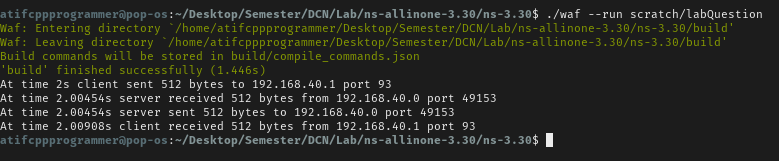
\includegraphics[width=\linewidth]{labQuestion.png}
  \caption{labQuestion.cc}
  \label{fig:output2}
\end{figure}

\section{Conclusions}
NS-3 allows us to model and analyze a given network.

\section{Post-Lab Question}
The Code and its accompanying output is presented below.
\begin{verbatim}

#include "ns3/core-module.h"
#include "ns3/network-module.h"
#include "ns3/internet-module.h"
#include "ns3/point-to-point-module.h"
#include "ns3/applications-module.h"

using namespace ns3;

NS_LOG_COMPONENT_DEFINE ("atifcppprogrammer_post_lab");

int
main (int argc, char *argv[])
{
  CommandLine cmd;
  cmd.Parse (argc, argv);

  Time::SetResolution (Time::NS);
  LogComponentEnable ("UdpEchoClientApplication", LOG_LEVEL_INFO);
  LogComponentEnable ("UdpEchoServerApplication", LOG_LEVEL_INFO);

  // Creating Node Container for Our Two Client Nodes and One Server Node.
  NodeContainer allNodes;
  allNodes.Create(3);

  // Node Container for first Client-Server Point to Point Link.
  NodeContainer nodesOne;
  nodesOne = NodeContainer(allNodes.Get(0),allNodes.Get(1));

  // Node Container for second Client-Server Point to Point Link.
  NodeContainer nodesTwo;
  nodesTwo = NodeContainer(allNodes.Get(1),allNodes.Get(2));

  // Specifying PointToPoint Link for nodesOne Container.
  PointToPointHelper pointToPointOne;
  pointToPointOne.SetDeviceAttribute("DataRate",StringValue("8Mbps"));
  pointToPointOne.SetChannelAttribute("Delay",StringValue("8ms"));

  // Specifying PointToPoint Link for nodesTwo Container.
  PointToPointHelper pointToPointTwo;
  pointToPointOne.SetDeviceAttribute("DataRate",StringValue("4Mbps"));
  pointToPointOne.SetChannelAttribute("Delay",StringValue("4ms"));

  // Installing Network-Cards on nodesOne.
  NetDeviceContainer devicesOne;
  devicesOne = pointToPointOne.Install(nodesOne);

  // Installing Network-Cards on nodesTwo.
  NetDeviceContainer devicesTwo;
  devicesTwo = pointToPointTwo.Install(nodesTwo);

  // Installing Protocol Stack on First Client and Server;
  InternetStackHelper stackOne;
  stackOne.Install(nodesOne);

  // Installing Protocol Stack on Second Client.
  InternetStackHelper stackTwo;
  stackTwo.Install(nodesTwo.Get(1));

  // Specifying and Assigning IP-Addresses for First Client and Server Link.
  Ipv4AddressHelper addressOne;
  addressOne.SetBase ("192.168.1.0", "255.255.255.0","0.0.0.1");

  Ipv4InterfaceContainer interfacesOne = addressOne.Assign (devicesOne);

  // Specifying and Assigning IP-Addresses for Server and Second Client Link.
  Ipv4AddressHelper addressTwo;
  addressTwo.SetBase ("192.168.5.0", "255.255.255.0","0.0.0.1");

  Ipv4InterfaceContainer interfacesTwo = addressTwo.Assign (devicesTwo);

  // Installing UdpEchoServer on Central Node.
  UdpEchoServerHelper echoServer (9);

  ApplicationContainer serverApps = echoServer.Install (nodesOne.Get(1));
  serverApps.Start (Seconds (1.0));
  serverApps.Stop (Seconds (15.0));

  // Configuring and Installing First Client App.
  UdpEchoClientHelper echoClientOne (interfacesOne.GetAddress (1), 9);
  echoClientOne.SetAttribute ("MaxPackets", UintegerValue (1));
  echoClientOne.SetAttribute ("Interval", TimeValue (Seconds (1.0)));
  echoClientOne.SetAttribute ("PacketSize", UintegerValue (512));

  ApplicationContainer clientAppsOne = echoClientOne.Install (nodesOne.Get (0));
  clientAppsOne.Start (Seconds (5.0));
  clientAppsOne.Stop (Seconds (15.0));

  // Configuring and Installing Second Client App.
  UdpEchoClientHelper echoClientTwo (interfacesTwo.GetAddress (0), 9);
  echoClientTwo.SetAttribute ("MaxPackets", UintegerValue (1));
  echoClientTwo.SetAttribute ("Interval", TimeValue (Seconds (1.0)));
  echoClientOne.SetAttribute ("PacketSize", UintegerValue (512));

  ApplicationContainer clientAppsTwo = echoClientTwo.Install (nodesTwo.Get (1));
  clientAppsTwo.Start (Seconds (10.0));
  clientAppsTwo.Stop (Seconds (15.0));

  Simulator::Run ();
  Simulator::Destroy ();
  return 0;
}
\end{verbatim}

\begin{figure}[h!]
  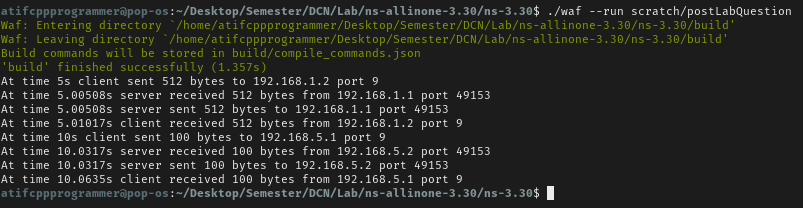
\includegraphics[width=\linewidth]{postLabQuestion.png}
  \caption{postLabQuestion.cc}
  \label{fig:output2}
\end{figure}

\end{document}
